Tato kapitola se věnuje rešerši existujících aplikací, které se zaměřují na elektronizaci třídních knih. Na trhu existuje celá řada řešení. Vybrané aplikace zde budou podrobněji popsány, budou uvedeny klady a zápory jednotlivých systémů a bude provedeno jejich srovnání. Rešerše  bude zaměřena především na funkce systému, cenu, uživatelské rozhraní a podporu.

\section{Etřídnice}
Prvním vybraným řešením je aplikace Etřídnice \cite{etridnice}. Tu provozuje společnost just4web.cz s.r.o. a pro školní agendu ji využívá 75 400 uživatelů.

Tento školský informační systém je rozdělen do modulů, kde třídní kniha je jedním z nich. Dalším modulem je například žákovská knížka, rozvrh hodin, deník praxe a úkoly.

\subsection{Funkcionalita a rozhraní}
Modul třídní kniha plnohodnotně nahrazuje klasickou třídní knihu a obsahuje následující funkce: 

\begin{itemize}
    \item zápis předmětu a učiva,
    \item zápis absence žáků,
    \item hospitace a inspekce,
    \item zápis projektů,
    \item zápis akcí a kurzů,
    \item přehled zameškaných hodin (omluvených/neomluvených),
    \item přehled odučených hodin učitelů,
    \item tisk všech přehledů, jako v klasické třídní knize,
    \item přístup pro rodiče a žáky k absenci,
    \item možnost posílání e-mailu rodičům při absenci jejich dětí.
\end{itemize}

\noindent Uživatelské rozhraní je intuitivní a kvalitně zpracované. Na obrázku \ref{etridnice} lze vidět ukázku aplikace. Konkrétně zápis předmětu a učiva do třídní knihy. Aplikace se skládá z hlavičky, navigačního menu a hlavní sekce. V hlavičce se nachází informace o přihlášeném uživateli a vyhledávací lišta. V navigačním menu lze přepínat mezi jednotlivými moduly a funkcemi, i zde se nachází informace o uživateli. Hlavní sekce se mění podle vybrané funkce a probíhá v ní užitečná práce, např. zápis učiva, absence, hospitace, atd.

\begin{figure}[h]
	\centering
	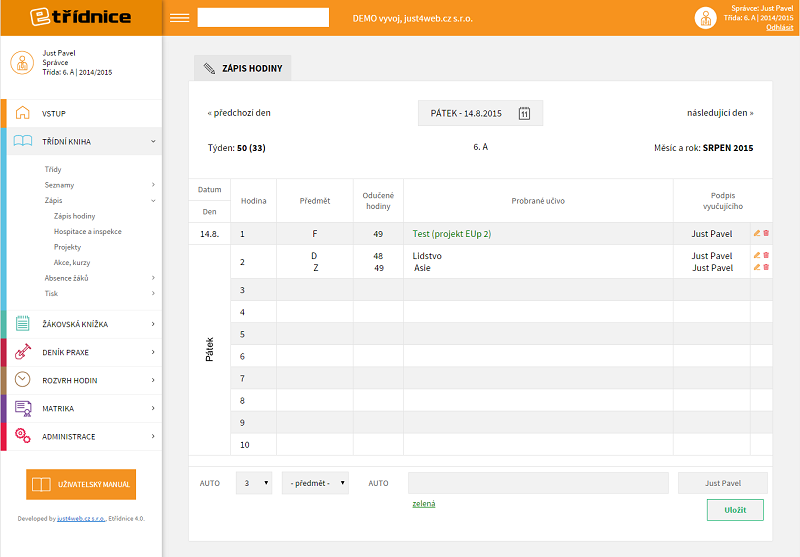
\includegraphics[width=\textwidth]{images/etridnice.png}
	\caption{Ukázka uživatelského rozhraní Etřídnice \cite{etridnice}}
	\label{etridnice}
\end{figure}

\subsection{Podmínky použití}
Cena se odvíjí od velikosti školy, respektive počtu žáků ve škole a platí se za roční licenci. Pohybuje se od 3~600 Kč pro počet žáků do 50, do 15~000~Kč, kde počet žáků může být až 1~000. V licenci jsou zahrnuty všechny moduly, včetně instalace a konfigurace systému, zálohování, aktualizací a uživatelské podpory. Ceny jsou uvedeny bez DPH. \cite{etridnice-cena} 

Systém Etřídnice je webová aplikace, jejíž hostování zajišťuje společnost just4web.cz s.r.o. Data, která aplikace ukládá, jsou umístěna na serveru poskytovatele, který je registrován u Úřadu pro ochranu osobních údajů. Pro přístup k nim se využívá protokol HTTPS, který se šifruje pomocí SSL. \cite{etridnice-podpora}

\subsection{Podpora}
Na webových stránkách Etřídnice nalezneme přehledný manuál k aplikaci. Ten je rozdělen na kapitoly, kde každému modulu je věnována právě jedna kapitola. Na stránkách najdeme i krátká videa, která demonstrují práci se systémem.

Společnost dále nabízí školení pro učitele či správce systému. Tato školení jsou však zpoplatněna. Cena za školení trvající dvě hodiny je 1 200 Kč.

\subsection{Identifikované klady a zápory}
Kladnými body řešení může být kvalitně zpracované uživatelské rozhraní, přehledný manuál a nižší cena oproti konkurenční aplikaci Edookit.

Naopak zápornými body může být nutnost uložení dat u poskytovatele a také fakt, že systém je sice rozdělen na moduly, ale licence, kterou je nutné zakoupit, obsahuje vždy všechny moduly. Není tedy možné vybrat si pouze určitý výčet modulů a platit například nižší cenu za licenci.

\section{Bakaláři}
Nejrozšířenější řešení v ČR je systém Bakaláři od společnosti BAKALÁŘI software s.r.o. \cite{bakalari}. Tento program používá přes milion uživatelů v ČR \cite{bakalari}. Stejně jako předchozí systém je i tento logicky rozdělen na moduly. Třídní kniha je jedním z modulů. Dalšími moduly, které řešení obsahuje, jsou například žákovská knížka, evidence žáků a zaměstnanců či modul pro přijímací zkoušky, knihovnu a inventarizaci.

\subsection{Funkcionalita a rozhraní}
Modul pro správu třídních knih plně nahrazuje třídní knihy v papírové podobě. V tomto modulu najdeme následující funkce:

\begin{itemize}
    \item zápis jednotlivých hodin,
    \item zápis nepřítomnosti žáků,
    \item omlouvání absence třídním učitelem,
    \item tiskové výstupy,
    \item poznámky o zadání domácího úkolu,
    \item zobrazení pořádkové služby,
    \item hospitace,
    \item poučení o bezpečnosti práce,
    \item specifická data žáků -- např. informaci o tom, že dojíždí,
    \item kontrola zapsaných hodin -- např. před archivací zkontrolovat, zdali něco nechybí,
    \item kontrola absencí.
\end{itemize}

\noindent Společnost nabízí pro přístup do systému tři řešení. Jedná se o desktopovou aplikaci, která je nainstalována na počítačích ve škole, webovou aplikaci a mobilní aplikaci.

Obrázek \ref{bakalari1} zobrazuje ukázku desktopové aplikace. Uživatelské rozhraní není moderní ani uživatelsky přívětivé. Zápis do třídní knihy probíhá přes nové okno, kde se vyplní téma hodiny, absence žáků apod. Informace o hodině se vyplní automaticky díky modulu rozvrhu a suplování. Bez tohoto modulu společnost nedoporučuje používat modul pro třídní knihu.

\begin{figure}[H]
	\centering
	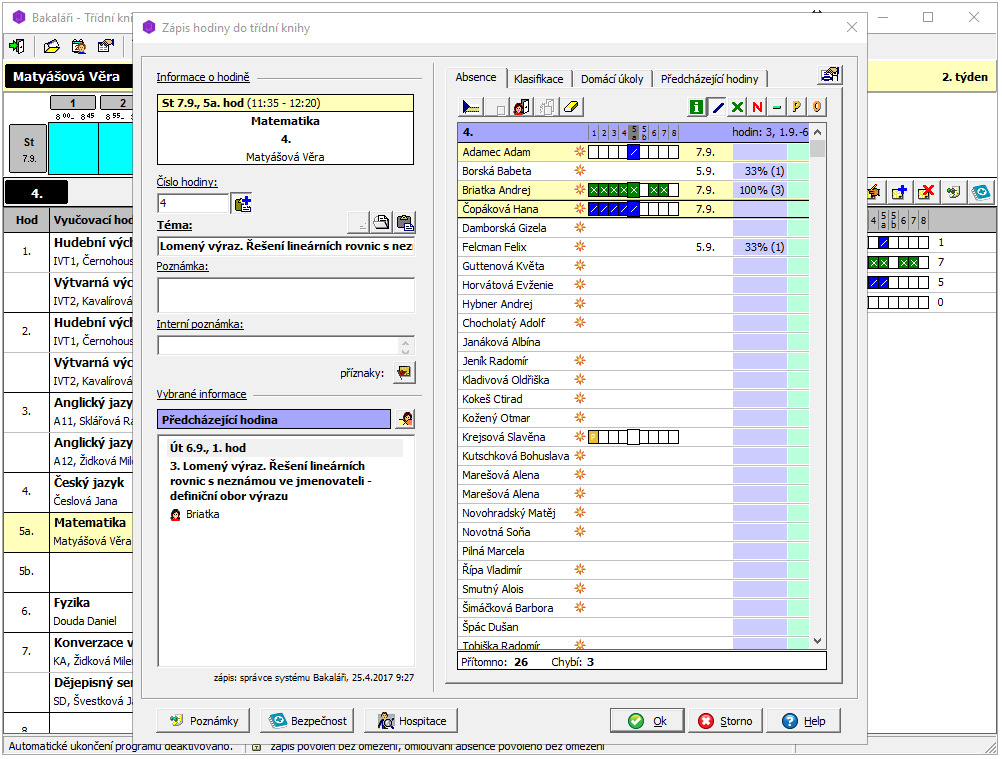
\includegraphics[width=\textwidth]{images/bakalari1.png}
	\caption{Desktopová aplikace systému Bakaláři \cite{bakalari}}
	\label{bakalari1}
\end{figure}

Na obrázku \ref{bakalari2} lze vidět ukázku webové aplikace Bakaláři. V tomto případě je uživatelské rozhraní již přívětivější. Aplikace je rozdělena na tři části. Hlavičku, která je umístěná nahoře a obsahuje informace o přihlášeném uživateli. Navigační menu, umístěné na levé straně aplikace, které slouží k přepínání na jednotlivé funkce. Hlavní část, kde probíhá užitečná práce se systémem.

\begin{figure}[h]
	\centering
	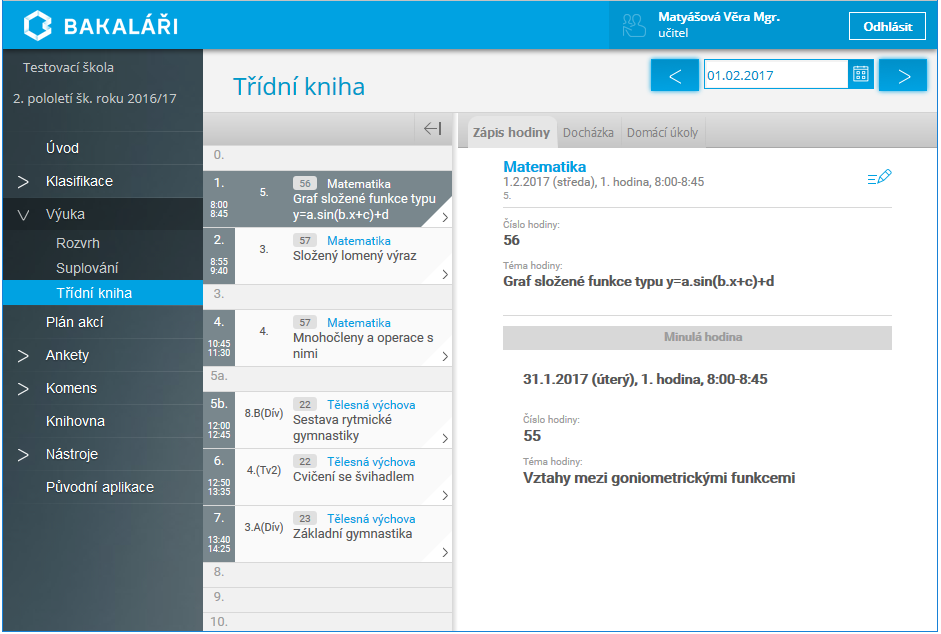
\includegraphics[width=\textwidth]{images/bakalari2.png}
	\caption{Webová aplikace systému Bakaláři}
	\label{bakalari2}
\end{figure}


\subsection{Podmínky použití}
Cena se stejně jako u předchozího systému odvíjí od velikosti školy a platí se za roční pronájem licence. Je možnost zakoupit pouze některé moduly, není tedy nutnost kupovat všechny. Přesná cena, či rozsah není zveřejněn.

Společnost BAKALÁŘI software s.r.o. umožňuje tři způsoby provozu aplikace. 
První možnost je provoz ve školní síti. Zde je aplikace provozována na virtuálním nebo fyzickém serveru školy. Výhoda tohoto řešení je především to, že vše je uloženo ve škole. Nevýhodou je nutnost pořídit server a licenci pro MS Server a nutnost udržovat provoz serveru. \cite{bakalari_nasazeni}

Druhá možnost je provozovat systém plně v cloudu poskytovatele. Výhodou u tohoto způsobu je, že není nutné pořizovat server ani licenci, vše je v režii poskytovatele. Nevýhodou může být svěření dat poskytovateli, měsíční platby za cloud či nutnost internetu k přístupu do systému. \cite{bakalari_nasazeni}

Poslední možností je kombinace dvou předchozích. V tomto případě je systém Bakaláři nainstalován na souborovém serveru školy, webová aplikace a data jsou pak v cloudu poskytovatele. Hlavní výhodou je, že webová aplikace běží nezávisle na škole, případný výpadek konektivity ve škole neovlivní přístup rodičů a žáků. Další výhodou je, že není nutné vlastnit a provozovat fyzický server s MS Server operačním systémem. Nevýhodou jsou opět měsíční poplatky za cloud, data u poskytovatele a nutnost internetového připojení pro provoz. \cite{bakalari_nasazeni}

\subsection{Podpora}
Společnost poskytuje návod na obsluhu systému na svých webových stránkách a krátká videa demonstrující některé funkcionality na platformě YouTube.

Co se týče technické podpory, společnost nabízí mailovou podporu bez analýzy dat a telefonickou podporu v pracovní době bez připojení přes vzdálenou plochu zdarma. Další služby jsou již zpoplatněny a jsou rozděleny do tří skupin. Jedná se o standardní služby, kam patří například analýza problému ze zaslaných dat či obnova dat ze zálohy. Zde je hodinová sazba nastavena na 1 200 Kč/hod. Pokud se však zjistí, že problém nevznikl na straně školy, jsou i tyto služby zdarma. Druhá skupina jsou individuální služby. Ty se objednávají až měsíc dopředu a cena je dohodnutá předem při objednávce a posouzení složitosti zásahu. Mezi tyto služby patří například převod dat z jiných systémů či tvorba rozvrhu na zakázku. Třetí skupinou je tzv. služba PODPORA+. Jedná se o doplňkovou službu k zakoupené licenci v podobě nadstandardní technické podpory. Jedná se například o přednostní odbavení telefonních hovorů, vzdálenou podporu TeamViewer či instalaci SQL serveru.

Veškerou placenou podporu zajišťují buď pracovníci společnosti Bakaláři software s.r.o. nebo certifikovaní konzultanti.

\subsection{Identifikované klady a zápory}
U řešení Bakaláři může být kladným bodem možnost vybrat si, kde bude aplikace provozována a kde budou uložena data. Další výhodou může být rozdělení do modulů podle funkcionalit a kvalitní podpora. V tomto případě lze zakoupit pouze určitý výčet modulů.

Nevýhodou je špatně zpracované uživatelské rozhraní u desktopové aplikace. Cena systému není zveřejněna, což znemožňuje tvořit v tomto směru objektivní závěr.

\section{Edookit}
Řešení Edookit od stejnojmenné firmy Edookit s.r.o. je kompletní informační systém pro mateřské, základní, střední a vyšší odborné školy \cite{edookit}. Tuto aplikaci využívá 350 000 aktivních uživatelů. Systém běží v cloudu a obsahuje funkcionalitu pro třídní knihu, žákovskou knížku, matriku, tvorbu rozvrhu, administrativu školy a komunikaci se studenty, rodiči a kolegy. 

\subsection{Funkcionalita a rozhraní}
Elektronická třídní kniha v tomto řešení umožňuje:

\begin{itemize}
    \item zapisovat a omlouvat absenci žáků,
    \item zapisovat probrané učivo,
    \item vkládat úkoly na příští hodinu,
    \item mít seznam žáků ve třídě nebo předmětu a jejich zasedací pořádek,
    \item vytvářet či měnit tematické plány,
    \item hodnotit žáky pomocí známek, procent či slovním hodnocením,
    \item sestavovat multimediální obsah z textu, obrázku, online testů, apod.,
    \item sdílet informace s vybranými skupinami či jednotlivci.
\end{itemize}

Aplikace je přístupná jak z webového prohlížeče, tak z mobilní aplikace. Uživatelské rozhraní je přehledné a intuitivní. Na obrázku \ref{edookit} lze vidět rozhraní aplikace Edookit. Aplikace se skládá z hlavičky nahoře, kde jsou odkazy na hlavní části aplikace a informace o přihlášeném uživateli, a z hlavní sekce, kde nahoře jsou odkazy na jednotlivé funkcionality a pod nimi již samotný obsah aplikace.

\begin{figure}[h]
	\centering
	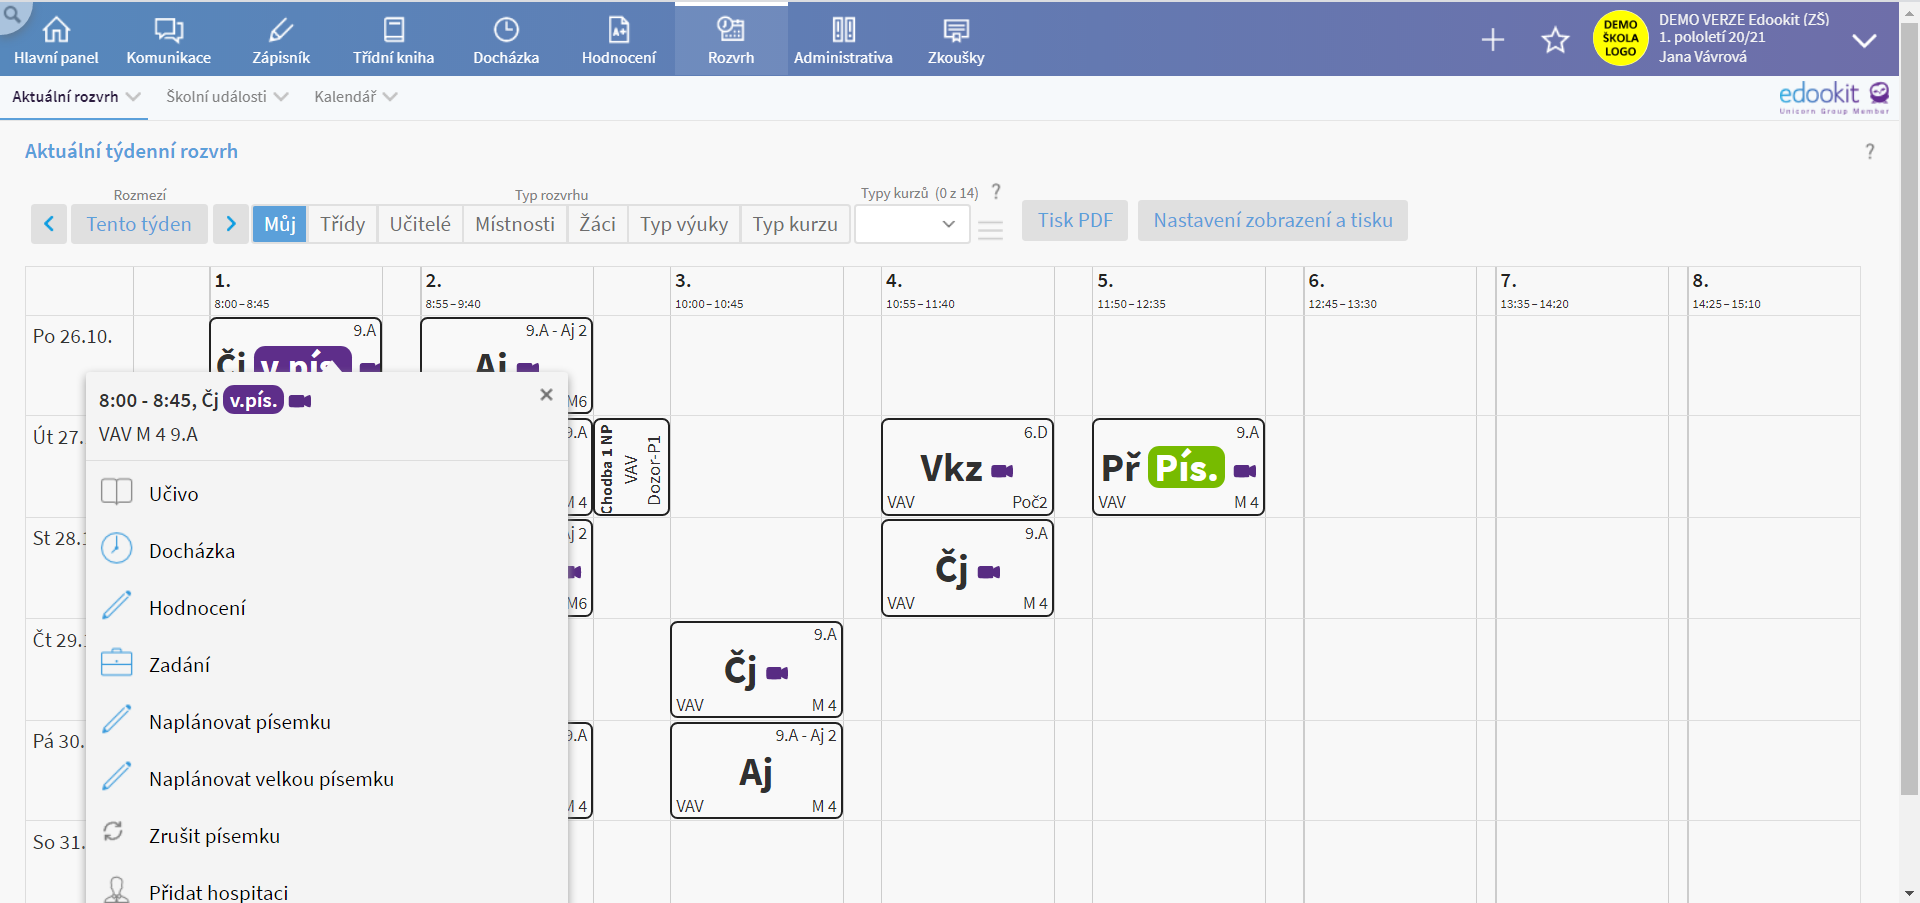
\includegraphics[width=\textwidth]{images/edookit.png}
	\caption{Ukázka uživatelského prostředí Edookit \cite{edookit}}
	\label{edookit}
\end{figure}

\subsection{Podmínky použití}
Systém není cenově rozdělen na moduly, cena zahrnuje celý informační systém. Cena se i zde odvíjí od velikosti školy, resp. počtu žáků a platí se za roční provoz. Pro mateřské, základní a střední školy se cena pohybuje od 14 400~Kč pro počet žáků do 100, do 79 900 Kč pro počet žáků do 1 000. Pro vyšší odborné školy je cena vyšší. Pohybuje se od 24 000 Kč pro počet studentů do 100, do 187 200 Kč pro počet studentů menší než 1 000. Cena je uvedena včetně DPH 21\% a zahrnuje provoz aplikace, aktualizace, datový prostor 100~GB, technickou podporu a zálohování. Instalační poplatek zahrnující vložení školy do systému, import dat, počáteční nastavení a úvodní školení pro učitele je stanoven na 3 000 Kč vč. DPH.

Edookit je webová aplikace, jejíž hostování zařizuje společnost Edookit s.r.o. Podle obchodních podmínek \cite{edookit-podminky} jsou data \uv{\textit{ukládána a spravována v souladu s Nařízením Evropského parlamentu a Rady (EU) 2016/679 o ochraně fyzických osob v souvislosti se zpracováním osobních údajů a o volném pohybu těchto údajů a o zrušení směrnice 95/46/ES (obecné nařízení o ochraně osobních údajů, dále jen Nařízení GDPR)}}.

\subsection{Podpora}
Společnost na svých webových stránkách poskytuje návody ve formě PDF pro jednotlivé funkce a úkony. Mají také zveřejněnou nahrávku ze školení pro učitele. Dále nabízejí zpoplatněné služby jako například navýšení datového prostoru, nadstandardní školení či vývoj speciální nové funkce. Na webových stránkách poskytují odkaz na demo verzi, kde je možné systém zdarma vyzkoušet.

\subsection{Identifikované klady a zápory}
U řešení Edookit jsou kladným bodem kvalitně zpracované návody.

Nedostatkem tohoto řešení je především absence rozdělení funkcionalit na moduly, což znamená, že škola musí platit za celý systém, i když chce využívat například jen zlomek funkcionalit. Další nevýhodou je cena, která je oproti konkurenčnímu řešení Etřídnice vyšší. Pro některé školy může být také překážka to, že data musí být uložena pouze u poskytovatele a ne na školním serveru. Poslední nalezenou nevýhodou může být uživatelské rozhraní, které není z pohledu autora této práce příliš intuitivní a je potřeba si nastudovat uživatelskou příručku. 

\section{Srovnání}
V této kapitole byla provedena rešerše třech systémů, které řeší problém elektronizace třídních knih. Všechna zkoumaná řešení mají své silné a slabé stránky, které jsou uvedeny v jednotlivých podkapitolách. Ať už si škola vybere jakýkoliv zmíněný systém, nevyhne se kompromisům. Těmi mohou být například:

\begin{itemize}
    \item uživatelské rozhraní (Bakaláři, Edookit),
    \item nutnost pořídit celý systém, ne pouze výčet modulů (Etřídnice, Edookit),
    \item data uložená pouze u poskytovatele (Etřídnice, Edookit),
    \item cena (Edookit).
\end{itemize}

\noindent Všechny aplikace nabízejí víceméně stejnou základní funkcionalitu pro správu třídních knih. Rozdíly jsou především v uživatelském rozhraní, provozu aplikace a cenové politice.

Funkcionalita je u všech řešení logicky rozdělena do funkčních celků, kde třídní kniha je jednou z nich. Dále nabízejí žákovské knížky, matriku, rozvrhy, přístup pro rodiče a další. Řešení Bakaláři nabízí modul pro přijímací zkoušky a inventarizaci, což konkurenční aplikace nenabízí.

Uživatelské rozhraní je dalším rozdílem uvedených systémů. Kvalitně zpracovaným uživatelským rozhraním, které je zároveň intuitivní, disponuje aplikace Etřídnice. Naopak u aplikací Edookit a Bakaláři je intuitivnost rozhraní menší.

Další rozdíly lze vidět i v provozu systému. Zde vyniká řešení Bakaláři, které nabízí tři druhy provozu -- ve školní síti, v cloudu poskytovatele a kombinaci předchozích dvou. Oproti tomu aplikace Edookit a Etřídnice nabízí pouze provoz u poskytovatele.

Poslední rozdíl je v cenové politice společností. U systémů Etřídnice a Edookit nelze platit pouze za výčet funkcionalit systému a je potřeba si pořídit celý systém. Řešení Bakaláři se v tomto ohledu odlišuje, zde společnost nabízí možnost platit pouze za některé moduly.
Konkrétní ceny jsou zveřejněné pouze u systémů Etřídnice a Edookit. Zde je levnější řešení Etřídnice, kde se za roční licenci platí 3 600 -- 15 000 Kč bez DPH. U řešení Edookit se roční cena pohybuje mezi 11 900 -- 154 710 Kč bez DPH.
